\RequirePackage[l2tabu, orthodox]{nag} 					% Checks for obsolete syntax and package % Layout
\documentclass[10pt,a4paper]{article} 					% KOMA-Script article scrartcl
\usepackage[nochapters]{classicthesis} 					% nochapters
\usepackage[top=2.5cm, bottom=2.5cm, left=4cm, right=4cm]{geometry} %Margins
%% Math
\usepackage{mathtools} 									% math
\usepackage{amsthm} 									% theorems and definition
\usepackage[all,error]{onlyamsmath}
%% Figures and tables
\usepackage{booktabs} 									% pretty tables
\usepackage{subcaption} 								% subfigures
\usepackage{pgfplots,tikz} \pgfplotsset{compat =1.11} 	% figures
\usetikzlibrary{decorations.pathreplacing}
%% References
\usepackage{hyperref}  									% hypersetup
\usepackage{cleveref} 									% auto-detect cross reference type when using \cref
% bibliography
\usepackage{csquotes}
\emergencystretch=1em
\usepackage[%
backend=bibtex,   										% use BibTeX
style=chicago-authordate,
natbib=true,
bibwarn=true,
backref=true,
url=false, isbn=false
]{biblatex}
\addbibresource[datatype=bibtex]{../../bib/library.bib}
%% Misc.
\usepackage{microtype} 									% improves the spacing between words and letters
\usepackage[colorinlistoftodos]{todonotes} 				% todo notes
\usepackage{url} 										% for line breaks in url links
\usepackage[titletoc,toc,title]{appendix} 				% appendices
\usepackage{accents} 									% underbar
\newcommand{\ubar}[1]{\underaccent{\bar}{#1}}
% other configurations
%%--------------------------------------------------------------------------
%% Colors and hypersetup
%%--------------------------------------------------------------------------
\hypersetup{
	colorlinks = true,      					%	Color links instead of ugly boxes
	urlcolor   = webbrown,  					%	Colors for external hyperlinks
	linkcolor  = blue,      					%	Colors of internal links
	citecolor  = webgreen,						%	Colors of citations
	pdfauthor = {Rud Faden: rudfaden@gmail.com},
	pdfcreator = {LaTeXing}
}

%%--------------------------------------------------------------------------
%% Theorem & Definitions
%%--------------------------------------------------------------------------

% Theorem Styles
\newtheorem{thm}{Theorem}[section]
\newtheorem{lemma}[thm]{Lemma}
\newtheorem{prop}[thm]{Proposition}
\newtheorem{corollary}[thm]{Corollary}
\newtheorem{assumption}[thm]{Assumption}
% Definition Styles
\theoremstyle{definition}
\newtheorem{defn}{Definition}[section]
\newtheorem{example}{Example}[section]
\theoremstyle{remark}
\newtheorem{remark}{Remark}


%%--------------------------------------------------------------------------
%% User specified LaTeX commands.
%%--------------------------------------------------------------------------

\global\long\def\argmax{\operatornamewithlimits{arg\, max}} % make the \argmax command available
\let\marginpar\oldmarginpar% fix for todonotes margin notes
\makeatletter
\DeclareRobustCommand{\pder}[1]{%
  \@ifnextchar\bgroup{\@pder{#1}}{\@pder{}{#1}}}
\newcommand{\@pder}[2]{\frac{\partial#1}{\partial#2}}
\makeatother
%%--------------------------------------------------------------------------
%% Misc
%%--------------------------------------------------------------------------

\setkeys{Gin}{width=1\textwidth} % make figures as wide as the margins
%solves wird tikz error
\makeatletter
\global\let\tikz@ensure@dollar@catcode=\relax
\makeatother
%%--------------------------------------------------------------------------
%% title and author
%%--------------------------------------------------------------------------

\title{\rmfamily\normalfont\spacedallcaps{Physician Information Acquisition In a Dynamic Setting}}
\author{\spacedlowsmallcaps{Rud Faden}}
\date{} % no date

\begin{document}

\maketitle

%%--------------------------------------------------------------------------
%% Abstract
%%--------------------------------------------------------------------------

\begin{abstract}
In this project, I examine provider and patient demand for information in a dynamic model where the diagnostic precision is assumed to be related to physician effort, and effort is non-contractible. In each period where the patient and physician interact, the physician gathers information about the patient, and the diagnostic precision is increased. Therefore, optimal physician effort decreases as the physician and patient tie increases. As the physician is unobserved, the insurer compensates the physician by the average effort in the physician population and physician will not provide an optimal level of diagnostic precision in the in the first encounters with a new patient. Therefore the switching cost of the patient increases as the tie with the physician lengthens. This model explains (i) why the cost is negatively related with patient, physician ties and (ii) also introduces the concept of an ``information trap'', where competition is deceasing in the patient physician tie as switching cost increases. Increases.
\end{abstract}

%%--------------------------------------------------------------------------
%% Section: The Patients Utility}
%%--------------------------------------------------------------------------

\section{The Patients Utility}

Following \citet{Rochaix1989}, the patient has a utility function
\[
	U = u(t,s):\, T\times S\rightarrow\mathbb{R}
\]
where \(t\) is treatment, \(s\) is disease variable classified by its severity of illness, where both \(t\) and \(s\) traverse a real line. It is assumed that the utility function has both increasing and decreasing parts to capture the negative effects of both under and over treatment. It is further assumed that the dis-utility of moving away from the optimum is increasing in \(s\)  such that the patient is more \emph{risk-sensitive} for higher values of \(s\)

%========== DEFINITION: Risk-sensitivity ==========%
\begin{defn}\label{def:risk-sensitivity}
Assuming that the decision problem has a unique solution \(t^{*}(s)\)  and for \(s'>s\),  \(u(t^{*}(s),s)=u(t^{*}(s'),s')\). Then for \(t^{*}(s)>t_{1}\), \(t^{*}(s')>t_{2}\),  \(t_{2}\ge t_{1}\), and \(t^{*}(s')-t_{2}=t^{*}(s)-t_{1}=\Delta t\) the \emph{risk-sensitivity} is monotonically increasing in \(s\)  if
\[
	0\le u(t^{*}(s),s)-u(t_{1},s)\le u(t^{*}(s'),s')-u(t_{2},s')\label{eq:risk-sensitivity}
\]
for all \(s\) and \(t\)  and I write that \(u(t_{1},s)\preceq u(t_{2},s')\)
\end{defn}
%==================================================%

The notion of \emph{risk-sensitivity} is illustrated in \cref{fig:The-patients-utility}.

%========== THEOREM: Single crossing property ==========%
\begin{thm}\label{thm:single-crossing}
If the risk sensitivity is increasing in \(s\)  then for \(s'>s\)  \(u(t,s)\) has a single crossing property in \((s,t)\)
\end{thm}
%==================================================%

%========== PROF - crossing property ==========%
\begin{proof}
Let \(t'=t^{*}(s')\) and \(t=t^{*}(s)\). Given \cref{def:risk-sensitivity}, it is clear that \(t'\ge t_{2}>t\ge t_{1}\). Therefore I can rewrite \cref{eq:risk-sensitivity} as
\begin{align}
  u(t',s')-u(t_{2},s')\ge u(t,s)-u(t_{1},s)\ge0\label{eq:increasing-differences}
\end{align}
\cref{eq:increasing-differences} clearly have increasing differences in \(s\) and thereby satisfies the single crossing property.
\end{proof}
%==================================================%

The intuition behind \cref{thm:single-crossing}, is that the marginal change \(u(t',\cdot)-u(t,\cdot)\) is larger, when \(s\) is larger. When \(u(t,s)\) is differentiable and concave as in \cref{fig:The-patients-utility}, one might note \(\partial u(t,s)/\partial t\ge0\) for \(t\le t^{*}(s)\) and that for \(\partial u(t,s)/\partial t\le0\) for \(t\ge t^{*}(s)\). Thereby \(\partial u(t,s')/\partial t>\partial u(t,s)/\partial t\) for \(t\le t^{*}(s)\) and \(\partial u(t,s')/\partial t<\partial u(t,s)/\partial t\) for \(t\ge t^{*}(s)\). One might also note that \(\partial u(t,s')/\partial t\) crosses \(\partial u(t,s)/\partial t\) at most once, and only from below.

%========== FIGURE: Utility and single-crossing ==========%
\begin{figure}
     \centering
    \begin{subfigure}[b]{0.49\textwidth}
		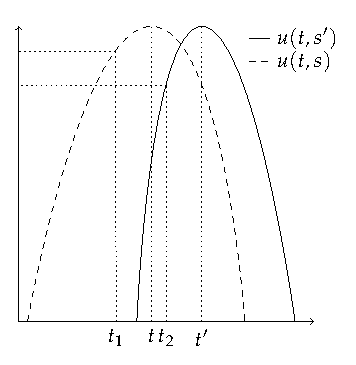
\includegraphics[width=\textwidth]{../fig/patient-utility.pdf}
	\end{subfigure}
    \begin{subfigure}[b]{0.49\textwidth}
		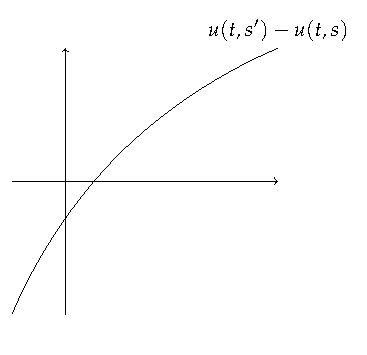
\includegraphics[width=\textwidth]{../fig/single-crossing-property.pdf}
	\end{subfigure}
\caption{\label{fig:The-patients-utility}The patients utility functions. If for the same change in \(t\) the loss in utility is smaller for \(s\) than for \(s'\)  when \(s<s'\)  then I says that risk sensitivity is increasing in \(s\) }
\end{figure}
%=======================================================%

%========== PROPOSITION: Single-crossing property ==========%
\begin{prop}
Given that \(u(t',s)-u(t,s)\) has a single crossing property in \(s\) and that both \(S\) and \(T\) are well ordered sets (in the strong set order)\footnote{If \(X' \geq X\) in the strong set order, then \(\max (x',x)\in X'\) and \(\min (x',x)\in X\). E.g. \([2,5]\geq[0,3]\) in the strong set order, while \(\{2,5\} \) and \(\{0,3\}\) is not.}, then
\[
	t^{*}(s)=\argmax_{s\in S}u(t,s)\label{eq:increasing-solution}
\]
is increasing in \(s\) \footnote{It should be noted that the assumption of quasi-supermodularity is not needed as the choice space is well ordered (e.i.\ a chain).}
\end{prop}

\begin{proof}
As both \(T\) and \(S\) are real lines, then it follows trivially that they are well ordered. For the rest of the proof see \textcite{Milgrom1994} or \cref{app:topiks-proof}
\end{proof}
%===========================================%

%========== EXAMPLE: Single-crossing ==========%
\begin{example}
A function with the properties defined in \cref{thm:single-crossing} and \cref{eq:risk-sensitivity} and have the form as in \cref{fig:The-patients-utility} is
\[
	u(t,s) = c-s{(s-t)}^{2}\label{eq:utility-example}
\]
where \(t,s\in\mathbb{R}^{+}\). Assuming that \cref{eq:utility-example} is continuous and twice differential in \(t,s\)  the derivative \(\partial^{2}u(t,s)\big/\partial t\partial s=2s^{2}\ge0\) and \cref{eq:utility-example} has increasing differences and thereby also a single crossing property in \((t,s)\)
\end{example}
%============================================%

%%--------------------------------------------------------------------------
%% Section: Uncertainty with perfect agency
%%--------------------------------------------------------------------------

\section{Uncertainty with perfect agency}

In reality however, \(s\) is never observed. The level of severity for the patients is a random variable represented by \(S\)  characterized by a subjective CDF. \(F(s)\)  with density \(f(s)\)  where \(s\) is a realization of \(S\). The expected value of choosing an admissible treatment intensity \(t\) is given by
\[
	u(t,S)=E[u(t,s)]=\max_{t}\int_{S}u(t,s)\, dF(s)\label{eq:expected-utility-prior}
\]
It is however possible to acquire costly information about \(s\) through medical diagnostics and physician effort. However, for two experiment \(X,Y\) on \(S\)  it is not a priori certain that one experiment \(X\) is necessary more \emph{informative} about \(s\) than the experiment \(Y\)  where \emph{informative} is to be understood in the way the posterior decision induced by the experiment \(X\) insures greater expected utility than the decision induced by the experiment \(Y\). Therefore we must introduce an order of information.

%%--------------------------------------------------------------------------
%% Section: Information ordering
%%--------------------------------------------------------------------------

\subsection{Information ordering}

%========== DEFINITION: affiliation ==========%
\begin{defn}\label{def:afflilation} \parencite{Milgrom1982}
For a family of density functions, let \(x\lor s\) denote the component wise maximum and \(x\land s\) the component wise minimum. Then \(x\) and \(s\) are affiliated if for all \(s\) and \(x\)
\[
	f(s\lor x)\, f(s\land x)\ge f(s)\, f(x)
\]
\end{defn}
%=============================================%

Affiliation of two random variables are equivalent to the monotone likelihood ratio property, and the intuition behind \cref{def:afflilation} is that higher signal realization of \(x\) makes the probability that \(s\) is large, higher. Similarly small signal realization of \(x\) makes the probability of a small \(s\) more likely.\footnote{See \cref{app:affiliation} for more details}

\textcite{Athey2002}  shows that solution given in \cref{eq:increasing-solution} is robust to uncertainty, such that
\[
	t^*(x)=\argmax_{s\in S, x\in X}\int_Su(t,s)\, dG^\eta(s\mid x)
\]
is increasing in \(x\)  whenever \(x\) and \(s\) are affiliated.\footnote{Note that here we, unlike in \cref{thm:informative}, consider the problem of deciding a treatment \(t\) before the state \(s\) is know, but \emph{after} observing the signal \(x\) }

%========== DEFINITION: Accuracy ==========%
\begin{defn}\label{def:accuracy}
\parencite{Persico2000} Given two signals (experiments) \(X^{\eta}\) and \(X^{\eta'}\),  \(X^{\eta'}\) is more accurate than \(X^{\eta}\) if
\[
	T_{\eta,s}(x)=F^{\eta'^{-1}}(F^{\eta}(x\mid s)\mid s)\label{eq:acuracy tranformation}
\]
is non decreasing in \(s\) for all \(x\)

Let \(E\) be a real line. A family of signals \(\left \{ X^{\eta}\right \} _{\eta\in E}\), with support \(X:=\bigcup_{x\in E}X^\eta\), is accuracy ordered (A-ordered) if a signal with higher index is more accurate than a signal with lower index.
\end{defn}
%================================================%

To understand the concept of accuracy, it can be noted that
\[
	T_{\eta,s}(X^{\eta}\mid s)\sim X^{\eta'}\mid s
\]
Thus a more accurate signal can be obtained from a less accurate signal, by the transformation \(T_{\eta,s}(X)\)  For a better understanding of the accuracy concept, see \cref{ex:t-transformation-1,ex:t-transformation-2}.

%========== EXAMPLE: T-transformation 1 ==========%
\begin{example}\label{ex:t-transformation-1}
Let  \(\eta\in[0,\infty]\) and let \(S\) be distributed according to any CDF and let \(X_{\eta}\sim\mathbb{U}(s-1/\eta,s+1/\eta)\) and let \(f(x\mid s)=\eta\big /2\) on \(X^\eta\). Then for \(\eta'>\eta\)
\[
	\frac{\eta'}{2}=\frac{\eta}{2}\left(T_{\eta,s}^{-1}(x)\right)'\Leftrightarrow T_{\eta,s}(x)=\frac{\eta}{\eta'}(x-s)+s
\]
To see why, note that

\begin{align*}
	T_{\eta,s}(x)^{-1}               &=\frac{\eta'+\eta s-s}{\eta} \Rightarrow \\
	\left(T_{\eta,s}(x)^{-1}\right)' &=\frac{\eta'}{\eta}
\end{align*}

\begin{figure}
	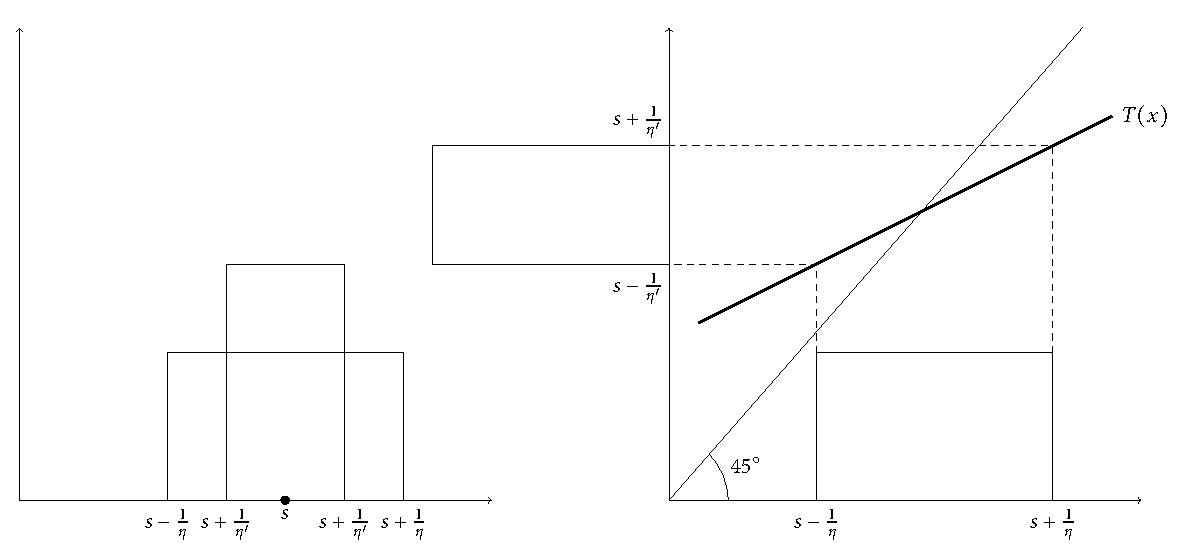
\includegraphics[width=\textwidth]{../fig/t-transformation.pdf}
	\caption{\label{fig:t-transformation}The \(T:{\eta,s}(x)\) transformation}
\end{figure}

Further, one might also note that \(T_{\eta,s}(x)\) is an increasing function by taking the derivative
\[
	\frac{\partial^2}{\partial \eta'\partial \eta}T_{\eta,s}(x)=\frac{\eta}{\eta'^2}>0
\]
Thus, \(T_{\eta,s}(x)\) transforms \(X^{\eta}\) into \(X^{\eta'}\) when \(T_{\eta,s}(x)\) is increasing. \citep{Persico1996}.

From \cref{fig:t-transformation}, the ting to note is that \(T_{\eta,s}(x)\) has a slope less than 1 and crosses the \(45^\circ\) line at \(s\). This means that \(T_{\eta,s}(x)\) contracts mass around \(s\). Further, observe that \(T_{\eta,s}(x)\) is a straight line passing through \((s,s)\). Thus increasing \(s\) to \(s'\) will course \(T_{\eta,s}(x)\) to shift up, so the line passes through \((s',s')\). Hence the notation of ``more accurate signal'' can be interpreted as one signal \(X^{\eta'}\) being more correlated with the ransom state \(s\) than another signal \(X^\eta\), and the function \(T_{\eta,s}(x)\) imposes this additional correlation.

\end{example}
%=======================================================%
An illustrative example can also be given by applying \cref{eq:acuracy tranformation} to hypothesis testing.

%========== EXAMPLE: T-transformation 2==========%
\begin{example}\label{ex:t-transformation-2}
Consider the case where \(s\) can take two values \(s_{1}<s_{2}\). Let \(X^{\eta}\) be a information structure affiliated with \(S\). The optimal test based on \(X^{\eta}\) is given by the rejection region \(X^{\eta}>x^{*}\)  such that \(s_{1}\) is rejected in favor of \(s_{2}\) when \(X^{\eta}>x^{*}\). The probability of a type I error is then \(\mathbb{P}(X^{\eta}\le x^{*})=F(x^{*}\mid s_{2})\) and the probability of a type II error is \(1-F(x^{*}\mid s_{1})\). Now given that \(X^{\eta'}\) is more accurate than \(X^{\eta}\) is is possible to design a test with the same probability of type I error, by choosing \(x^{**}\) such that \(F(x^{**}\mid s_{2})=F(x^{*}\mid s_{2})\) (e.i. \ accept \(s_{2}\) if \(X^{\eta}\ge x^{**}\) . However, since \(X^{\eta'}\) is more accurate than \(X^{\eta}\)  then \(x^{**}\ge F^{\eta'^{-1}}(F^{\eta}(x\mid s_{1})\mid s_{1})\). As \(x^{**}\) lies on or, to the right of \(x^{*}\) then the test based on \(X^{\eta'}\) is a least as powerful as the test based on \(X^{\eta}\) \citep{Lehmann1988,Persico2000}.\footnote{For a graphical example, see \cref{app:test-power}}
\end{example}
%=====================================================%

%%--------------------------------------------------------------------------
%% Subsection: Demand for information
%%--------------------------------------------------------------------------

\subsection{Demand for information}

Given that we now know, when a test can be considered more informative than another, I can know turn to the problem of informativeness. To use the notation of informativeness I make two assumptions

%==========  ASSUMPTION: needed for proof  ==========%
\begin{assumption}
	The utility function is differential in \(t\) and the optimal solution \(t^*(x)\) is differentiable in in \(\eta\) and \(x\)
\end{assumption}
\begin{assumption}
	For all pairs of signals and states \((s,x)\) the CDF \(G^\eta(s\mid x)\) is differentiable in \(\eta\) on \(E\) and is continuous in \(s\)
\end{assumption}
%====================================================%

%========== THEOREM: informative ==========%
\begin{thm}\label{thm:informative}
\parencite{Persico2000}
Suppose that \(X^{\eta}\) and \(X^{\eta'}\) are affiliated with \(S\) and that \(\left \{X^{\eta}\right \} _{\eta\in E}\) is A-ordered, such that \(X^{\eta'}\) is more accurate than \(X^{\eta}\). Then for all utility functions with a single crossing property, \(X^{\eta'}\) is more informative than \(X^{\eta}\)
\end{thm}
% the real important fact here is that u is monotonically increasing in s
\begin{proof}
See \citet{Lehmann1988} section 4 and \citet{Karlin1956} Lemma 3--4 and theorem 1.
\end{proof}
%=============================================%

It follows directly from \cref{thm:informative} that when \(X^{\eta'}\) is more informative than \(X^{\eta}\)  then
\begin{align}
	\label{eq:utility-increasing-information}
	\begin{split}
	\int_{X}\int_{S}u(t,s)\, dG^{\eta'}(s\mid x)\, dF(x)&\geq \int_{X}\int_{S}u(t,s)\, dG^{\eta}(s\mid x)\, dF(x) \Leftrightarrow \\
	U(t,s;\eta')&\geq U(s,t;\eta)
\end{split}
\end{align}

From the above equation, it is clear that the patient will always prefer a more accurate signal to a less accurate signal.

\cite{Persico2000} goes on to show that when \(u(t,s)\) is risk-sensitive increasing in \(s\), then the marginal value of information
\begin{align}
		MR(\eta)=\frac{\partial}{\partial \eta} \int_{X}\int_{S}u(t,s)\, dG^{\eta}(s\mid x)\, dF(x) \label{eq:marginal-value-of-information}
\end{align}


is increasing in \(s\).

From \cref{eq:marginal-value-of-information} it follows straight forward that the optimal level of accuracies defined by
\begin{align}
	MR(\eta)-C(\eta)=0
\end{align}
 is increasing in \(s\), where \(C(\eta)\) is the cost of obtaining the signal \(X^\eta\). In all of this paper it will be assumed that the cost of signal acquisition is increasing in \(\eta\), such that more accurate signals are more costly.
%%--------------------------------------------------------------------------
%% Section: The physician problem
%%--------------------------------------------------------------------------

\section{The physician problem}

The physician has a utility function given by
\[
	V=v(M,\eta)
\]
where the physicians payment, \(M\) is given by
\[
	M=\delta+(p-\omega)q
\]
where \(\delta\) is a fixed payment, \(p\) is the physician payment per unit of treatment, \(q\) is quantity of treatment.

I also assume that the physician can increase the quality of treatment by increasing the diagnosis accuracy through effort, such that \(\eta\) increases when more effort is applied. Where \(\eta\) is the level of accuracy in \(X^\eta\). The cost of accuracy is given by \(C\). Assuming a separable utility function, the physician problem can be expressed as
\[
	v(M,e)=M-C(\eta)
\]
As the subject of this paper, is the acquisition of information, through physician effort, I ignore the treatment decision and assume for simplicity that the payment for treatment \(p\) can be set exactly equal to the cost \(\omega\)  The problem then simplifies to
\begin{align}
v(\delta,\eta)=\delta-C(\eta)\label{eq:phys-utility}
\end{align}
Further, the physician will only apply effort as long as \cref{eq:phys-utility} is positive. Let \(\bar{\eta}\) be the solution to \(\delta=C(\eta)\). Then \(\bar{\eta}\) must be between \([0,\bar{\eta}]\).

If I let \(\lambda\in[0,1]\) be the physician preference for effort we can restate the physicians problem in \cref{eq:phys-utility} as
\begin{align*}
 	 v(\delta,\lambda,\bar{\eta})=\delta-C(\lambda\bar{\eta})\label{eq:phys-utility2}
\end{align*}

%%--------------------------------------------------------------------------
%% Section: The patients search for treatment in a static setting
%%--------------------------------------------------------------------------
\section{The patients search for the best treatment}

From \cref{eq:utility-increasing-information} it is clear that the patient will always prefer more information to less information. A optimal search strategy for the patient must then be to maximize \(\eta\)  To define the patients search, I assume that the patient knows the distribution of types \(\lambda\in \Lambda\)  \(Q(\lambda, \rho)\)  where \(\rho\) is parameter that indicates the dispersion of the market. In the first period, the patient consults a random physician and gets a utility of
\[
	u(t,S;\lambda)=\int_\Lambda\int_X\int_S u(t,s)\, dG^{\lambda\bar{\eta}}(s\mid x)\, dF(x)\, dQ(\lambda,\rho)
\]
In the next period, the patient has observed \(\lambda\). Further, the information obtained in the previous period \(\beta(\lambda\bar{\eta})_{i-1}\) about the patient is still available at the current physician, where \(\beta\) is the amount of information from the previous period that is still relevant in the current period. Therefore, the patient knows that he will get an expected utility of
\[
	u_{stay}(t,S;\lambda)=\int_X\int_S u(t,s)\, dG^{\beta\sum(\lambda\bar{\eta})_{i}}(s\mid x)\, dF(x)
\]
if he stays, and an expected utility of
\[
	u_{leave}(t,S;\lambda)=-C+\int_\Lambda\int_X\int_S u(t,s)\, dG^{\lambda\bar{\eta}}(s\mid x)\, dF(x)\, dQ(\lambda,\rho)
\]
if he leaves, where \(C\)  is the search cost.

It then follows that as the \(i\) increases \(u_{stay}\) will dominate \(u_{leave}\)
\begin{thm}
 	As \(i\) increases \(u_{stay}\) will dominate \(u_{leave}\) for some values of \(\beta\) and \(\lambda\)
\end{thm}
\todo[inline]{Herfra vil jeg gerne vise at n\aa r \(i\)  stiger, s\aa \  vil det altid v\ae re mere fordelagtigt for patienten at blive hos den samme l\ae ge (da informationen aggregers) end at finde en anden l\ae ge, selvom en ny l\ae ge m\aa ske er bedre (har h\o jre \(\lambda\) . S\aa ledes er der alts\aa \ en ``informations f\ae lde'', i og med at omkostnignerne ved at skifte er st\o rre end ved ikke at skifte, pga. informationen aggregeres.}
%%--------------------------------------------------------------------------
%% Dynamic Settings
%%--------------------------------------------------------------------------

\printbibliography%

%%--------------------------------------------------------------------------
%% Appendix
%%--------------------------------------------------------------------------

\begin{appendices}
\section{Appendix}\label{sec:appendix}
\subsection{More informative \& least as powerful test}\label{app:test-power}

See~\cref{fig:test-power}

\begin{figure}[!ht]
	\centering
	\begin{subfigure}[b]{\textwidth}
		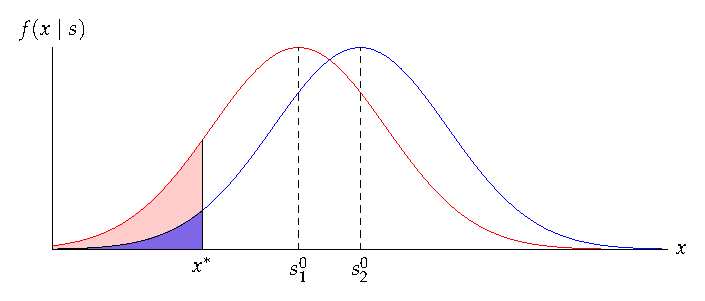
\includegraphics[width=\textwidth]{../fig/test-power-1.pdf}
		\caption{}\label{fig:test-power-1}
	\end{subfigure}
	\begin{subfigure}[b]{\textwidth}
		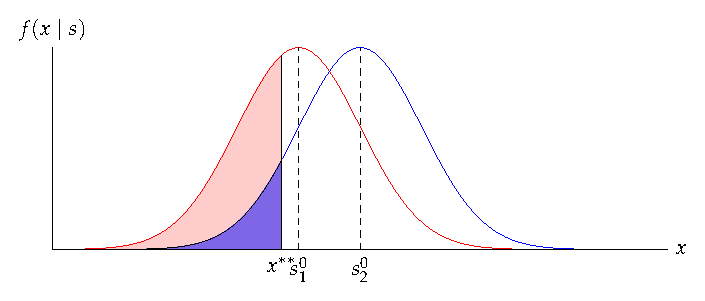
\includegraphics[width=\textwidth]{../fig/test-power-2.pdf}
		\caption{}\label{fig:test-power-2}
	\end{subfigure}
\caption{The blue shaded area is the probability of a type I error, and the red shaded area is the test power, while the non-shaded area under the red curve is the probability of a type II error. \Cref{fig:test-power-1,fig:test-power-2} have the same probability of a type I error, but the power of the test in \cref{fig:test-power-2} is higher than in \cref{fig:test-power-2}, as the probability of a type II error is smaller}\label{fig:test-power}
\end{figure}

%%--------------------------------------------------------------------------
%% Appendeix: Stochastic Affiliation
%%--------------------------------------------------------------------------

\subsection{Stochastic Affiliation}\label{app:affiliation}
\begin{defn}
	The random variables \(X_1,\ldots,X_n\) are said to be affiliated if their joint PDF \(f(\mathbf{x})\) is log-supermodular, meaning that for  all \(\mathbf{x},\mathbf{x}'\in\mathbb{R}_nb\), we have
	\[
		f(\mathbf{x}\land \mathbf{x}')f(\mathbf{x}\lor \mathbf{x}')\geq f(\mathbf{x})f(\mathbf{x}')
	\]
When \(f\) is twice continuously differentiable, then equivalently \(bX_1,\ldots,X_n\) are affiliated iff for all \(i\ne j\)
\[
	\frac{\partial^2}{\partial x_i \partial x_j}\ln f\geq 0
\]
\end{defn}
Consider two joint random variables \(X\) and \(S\). Affiliation then tells us about the conditional distribution of \(f(S\mid x)\). If \(x\leq x', y\leq y'\), then affiliation implies that
\[
	\frac{f(x,y')}{f(x,y)}\leq \frac{f(x',y')}{f(x'y)}
\]
which we can rewrite as
\[
	\frac{f(y'\mid x)f_X(x)}{f(y\mid x)f_X(x)}=\frac{f(y'\mid x)}{f(y\mid x)}\leq \frac{f(y'\mid x')}{f(y\mid x')} = \frac{f(y'\mid x')f_X(x')}{f(y\mid x')f_X(x')}
\]
which tells us the that likelihood ratio \(f(\cdot\mid x)\big/ f(\cdot\mid x)\) is increasing in \(x\) and thereby displays the monotone likelihood ratio property, which implies first-order (and hence second-order) stochastic dominance. \cite[in proposision 8 and 10 ]{Quah2009}, proofs that the monotone likelihood ratio property is required for the familiy of functions with the single-crossing property to have an increasing optimal solution in the signal \(x\).

%%--------------------------------------------------------------------------
%% Appendeix: Proof Topiks
%%--------------------------------------------------------------------------

\subsection[A simplified proof of Topkis’s Monotonicity Theorem is]{A simplified proof of \Citeauthor{Topkis1998}'s Monotonicity Theorem}\label{app:topiks-proof}
\begin{thm}
	Consider the problem
	\[
		t^*(s)=\argmax_{s\in S} u(t,s)
	\]
	where \(T,S\in \mathbb{R}\) and \(T_s\subset T\) is the correspondence from \(S\) to \(T\)  with \(T_s\) being the set of feasible treatments, when the diseases is \(s\)  Assume also that (i) \(u\) has increasing differences in \((t,s)\)  and (ii) \(T_s=[g(s),h(s)]\)  where \(h,g:S \rightarrow \mathbb{R}\) are increasing functions with \(g\leq h\).  Then the optimal solution \(t^*(s)\) is an increasing function.
\end{thm}

\begin{proof}
	The proof is done by contradiction. Assume that \(t^*(s)\) is not increasing. Then for some \(s'>s\)  \(t^*(s')<t^*(s)\).  Then using assumption (ii) and the fact that \(t^*(s)\in T_s\)  and \(t^*(s')\in T_{s'}\)  it follows that \(g(s)\leq g(s')\leq t^*(s') < t^*(s) \leq h(s) \leq h(s')\)  so that \(t^*(s)\in T_{s'}\) and \(t^*(s')\in T_s\).  Using the latter facts along with \(t^*(s)\in t(s)\) and \(t^*(s')\in t(s')\)  we have
	\[
		0\geq u[s',t^*(s)]-u[s',t^*(s')]\geq u[s,t^*(s)]-u[s,t^*(s')]\geq 0,
	\]
	which holds throughout. Hence, \(t^*(s)\in t(s')\) is a contradiction to the fact that \(t^*(s')=\max \{t(s')\}\)  since \(t^*(s')<t^*(s)\).  Hence, \(t^*(s)\) is an increasing function \parencite{Amir2005}.\footnote{In this proof, it is assumed that \(T_s\cap T_{s'}\ne \emptyset\). If this was the case, one would trivially have that \(t^*(s)<t^*(s')\) }
\end{proof}
\end{appendices}

\end{document}